\documentclass{beamer}
\usepackage{beamerthemesplit}
\usepackage{amsmath}
\usepackage{amssymb}
\usepackage{subfigure}
\usepackage{amsfonts}
\usepackage{newlfont}
\usepackage{graphics}
\usepackage{graphicx}
\usepackage{epsfig}
\usepackage[english]{babel}
%\usepackage[latin1]{inputenc}
\usepackage{wrapfig, blindtext}
\usepackage{multicol}
\usepackage{lmodern}
\usepackage{lipsum}
\usepackage{marvosym}
\usepackage{caption}

\usepackage[T1]{fontenc}
\usepackage{geometry}
\usepackage{latexsym}
\usepackage{algorithm}
\usepackage{algpseudocode}
\usepackage{comment}
%\usepackage{subcaption}
\usepackage{verbatim}
\usepackage{boxedminipage}
\usepackage{multirow}
\usepackage{color}


%\usepackage{hyperref}
%\usepackage[round]{natbib}

% \usetheme{default}
% \usetheme{Boadilla} %# not so good
% \usetheme{Madrid}  % # not so good
% \usetheme{Montpellier}
 \usetheme{Warsaw}
% \usetheme{Copenhagen}
% \usetheme{Goettingen}
% \usetheme{Hannover}
%\usetheme{Berkeley}
\usecolortheme{spruce}
%\beamertemplatesolidbackgroundcolor{craneorange!25}
%\setlength{\parskip}{8pt plus 1pt minus 1pt}
%\setbeamertemplate{footline}[frame number]
\bibliographystyle{unsrt}

%\title[IIITM Gwalior]{Title of the thesis}
%\author{Candidate name \\Candidate roll number}
%\vspace{0.7in}
%\begin{figure}
%
\includegraphics[height=1.25in,width=0.9in]{logo.pdf}\\
%\end{figure}\vspace{0.8in}
%\institute[]{
%
%ABV-Indian Institute of Information Technology and Management Gwalior,\\
%India
%}
%\date{\today}


\begin{document}
\begin{frame}
\begin{center}
{\bf \large{{\textup{\textbf{\textup{{Hospital Readmission Prediction Of ICU Patients Using Deep Learning Algorithms}}}}}}
\\[0.4in]}
by\\[0.2in]
{ {Shivam Sinha}}\\[0.1in]
{Roll. No.: 2014IPG-082}\\
\begin{figure}[ht]
\centering

\includegraphics[height=.8in,width=0.8in]{logo.pdf}\\
\end{figure}
{{\bf ABV--INDIAN INSTITUTE OF INFORMATION TECHNOLOGY AND MANAGEMENT GWALIOR (M.P.), INDIA\\[0.1in]}
}
\end{center}
\end{frame}
%\frame{\titlepage}


\begin{frame}{Introduction}
    \begin{itemize}
        \item A Hospital readmission is an episode when a patient who had been discharged from a hospital is admitted again within a specified time interval.
        \item Previously baseline classification models were used to estimate the Hospital Readmission Rates. Then Deep Neural Network (DNN) came into picture. A Deep Neural Network (DNN) is an Artificial Neural Network with multiple hidden layers between the input and output layers. Similar to shallow ANNs, DNNs can model complex non-linear relationships. It has been widely used in fields including computer vision, speech recognition, natural language processing, audio recognition, social network filtering, machine translation and bio-informatics where they produced results comparable to and in some cases superior to human experts.
    \end{itemize}
\end{frame}

\begin{frame}\frametitle{Motivation}
\begin{itemize}
\item For Medicare patients, hospitalizations can be stressful, even more so when they result in subsequent readmissions. A number of studies show that hospitals can engage in several activities to lower their rate of readmissions, such as clarifying patient discharge instructions, coordinating with post-acute care providers etc.
\item The purpose of this thesis is to use  deep neural networks which can work effectively to predict the result that can be utilized to avoid unnecessary hospital readmissions.
\end{itemize}
\end{frame}

\begin{frame}\frametitle{Key related research}

\begin{tabular}{ | p{1.5cm} | p{3.8cm} | p{5cm}| } 

\hline 
{\bf \begin{center} \footnotesize{Author (Year)} \end{center}} & {\bf \begin{center} \footnotesize{Paper Name} \end{center}} & {\bf \begin{center} \footnotesize{Comments} \end{center}} \\
\hline
\footnotesize{Ghassemi et al. (2014)} & \footnotesize{A data-driven approach to optimized medication dosing: a focus on heparin} & \footnotesize{An approach is developed that help clinicians determine the optimal initial dose of a drug to safely and quickly reach a therapeutic aPTT window.} \\ 
\hline
\footnotesize{Pirracchio et al.(2015)} & \footnotesize{Mortality prediction in intensive care units with the Super ICU Learner Algorithm (SICULA): a population-based study.} & \footnotesize{A super learner algorithm is used for predicting hospital mortality in patients.}\\
\hline
\footnotesize{Liang  and Hu (2015)} & \footnotesize{Recurrent convolutional neural network for object recognition} & \footnotesize{Combination of convolution and recurrent neural network model is used for object detection.}\\
\hline
\end{tabular}

\end{frame}


\begin{frame}\frametitle{Review of key related research}
\begin{tabular}{ | p{1.5cm} | p{3.8cm} | p{5cm}| } 

\hline 
{\bf \begin{center} \footnotesize{Author (Year)} \end{center}} & {\bf \begin{center} \footnotesize{Paper Name} \end{center}} & {\bf \begin{center} \footnotesize{Comments} \end{center}} \\
\hline
\footnotesize{Che et al.(2016)} & \footnotesize{Interpretable deep models for icu outcome prediction} & \footnotesize{Interpretable mimic learning is introduced that uses gradient boosting trees to learn interpretable models.}\\

\hline
\footnotesize{Jhonson et al. (2016) }& \footnotesize{MIMIC-III, a freely accessible critical care database} & \footnotesize{Medical Information Mart for Intensive Care (MIMIC-III) consists of data about patients admitted to various critical care units in a large hospital.} \\ 
\hline

\footnotesize{Hanson et al.} & \footnotesize{Improving protein disorder prediction by deep bidirectional long short-term memory recurrent neural networks} & \footnotesize{Long short term memory rnn in both directions is used to predict disordered proteins.}\\
\hline
\end{tabular}
\end{frame}


\begin{frame}\frametitle{Review of key related research}
\begin{tabular}{ | p{1.5cm} | p{3.8cm} | p{5cm}| } 

\hline 
{\bf \begin{center} \footnotesize{Author (Year)} \end{center}} & {\bf \begin{center} \footnotesize{Paper Name} \end{center}} & {\bf \begin{center} \footnotesize{Comments} \end{center}} \\
\hline
\footnotesize{Greff et al.(2017)} & \footnotesize{LSTM: A search space odyssey} & \footnotesize{Overcomes the vanishing gradient problem of traditional RNN.}\\


\hline
\footnotesize{Franco et al. (2017)} & \footnotesize{Impact of prealbumin on mortality and hospital readmission in patients with acute heart failure} & \footnotesize{Statistical Analysis is used to find the mortality and readmission rates.} \\ 
\hline
\footnotesize{Reddy and Delen (2018)} & \footnotesize{Predicting hospital readmission for lupus patients: An RNN-LSTM-based deep-learning methodology} & \footnotesize{ Utilizes deep learning methods to predict rehospitalization within 30 days by extracting the temporal relationships in the longitudinal EHR clinical data.}\\
\hline

\end{tabular}
\end{frame}



\begin{frame}{Research Gaps}
    In literature survey we find the following research gaps. These are points that we will
be focused on in this thesis.
    \begin{itemize}
        \item The results obtained in these techniques can be improved using novel classification algorithms. Most of the researchers have used existing machine learning algorithms and it is expected that deep learning techniques will surpass the conventional techniques.
        \item These previous works were not able to model high dimensional nonlinear relations as good as RNN.
        \item Descriptive statistics were being used in earlier methods. However, these statistics like mean, median & mode are always under the risk of loosing some vital
        information.
        \item Deep learning algorithms are still under shadow for variety of healthcare applications.
    \end{itemize}
\end{frame}

\begin{frame}{Extended Literature Survey}
\begin{tabular}{ | p{1.5cm} | p{3.8cm} | p{5cm}| } 

\hline 
{\bf \begin{center} \footnotesize{Author (Year)} \end{center}} & {\bf \begin{center} \footnotesize{Paper Name} \end{center}} & {\bf \begin{center} \footnotesize{Comments} \end{center}} \\
\hline
\footnotesize{Yang and Hossein Gandomi (2012)} & \footnotesize{Bat algorithm: a novel approach for global engineering optimization} & \footnotesize{Introduce a new natureinspired optimization algorithm, for solving engineering optimization tasks.}\\


\hline
\footnotesize{Mirjalili et al. (2014)} & \footnotesize{Grey Wolf Optimizer} & \footnotesize{Algorithm mimics the
leadership hierarchy and hunting mechanism of grey wolves in nature.} \\ 
\hline

\end{tabular}
\end{frame}

\begin{frame}{Suggestion of MTP Thesis Evaluation-I}
\begin{center}
\begin{tabular}{ | p{3cm} | p{7cm}| } 
\hline 
{\bf \begin{center} \footnotesize{Suggestion} \end{center}} & {\bf \begin{center} \footnotesize{Implementation/Improvement} \end{center}}\\
\hline
\footnotesize{Convolution vs Filter for feature extraction} & \footnotesize{Filters are mostly used in images to detect edges, lines etc. While convolution has weight to extract information. Since the dataset I am working on contains non-image data hence convolution is beign used for feature extraction.}\\ 
\hline
\footnotesize{Technique of the feature selection }& \footnotesize{Nature Inspired Algorithms are being used for feature selection i.e Bat Algorithm and Grey Wolf Optimizer Algorithm.}  \\ 
\hline
\footnotesize{Details of all Phases} & \footnotesize{Details of all phases like future extraction, algorithm implementation etc. have been included in the thesis report.}\\ 
\hline
\footnotesize{Rewrite Expected Results}& \footnotesize{Expected Results have been rewritten in the thesis report.}\\ 
\hline
\end{tabular}
\end{center}
\end{frame}

\begin{frame}\frametitle{Objectives}
The primary objective of this thesis is:
    \begin{itemize}
        \item To develop Deep Neural Network(DNN) models for Healthcare application i.e Hospital Readmission.
        \item To predict hospital readmission of patients using deep neural networks.
        \item To compare results between Deep Learning Models and with exiting algorithms.
    \end{itemize}
\end{frame}

\begin{frame}\frametitle{Novelty of the proposal}
    \begin{itemize}
        \item With this thesis, the aim is to use deep learning algorithms to overcome the drawbacks of conventional machine learning algorithms.
        \item The thesis aims to use nature inspired algorithms for feature extraction.
        \item The thesis also aims to use hybrid model (Convolution Recurrent Neural Network) which can further increase the accuracy of the proposed model.
    \end{itemize}
\end{frame}
\begin{frame}{Methodology\\\footnotesize{Flow Diagram}}
    \begin{figure}[h]
        \centering
        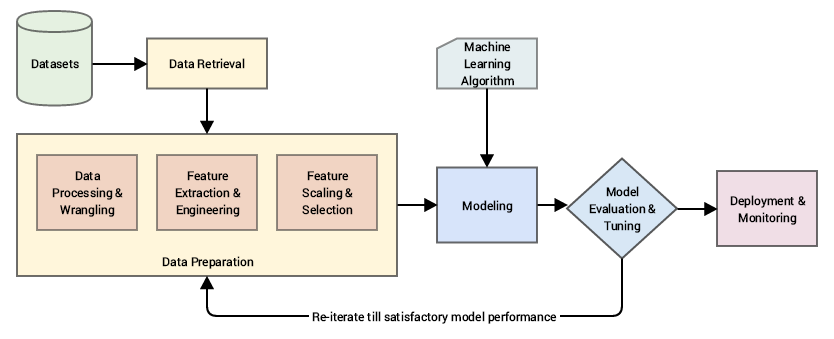
\includegraphics[width=4.5in]{flowdiag.png}
        \caption{Flow Diagram}
        \label{fig:flowdiag}
    \end{figure}
\end{frame}
\begin{frame}\frametitle{Methodology\\\footnotesize{Dataset Description}}
Medical Information Mart for Intensive Care (MIMIC-III)[\citenum{4}] consists of data about patients admitted to various critical care units in a large hospital.  A large number of different parameters
are present in MIMIC III database. These parameters include information such as vital signs, medications, laboratory measurements, observations, fluid balance, procedure
codes, diagnostic codes, imaging reports, hospital length of stay, survival data, and others. The database consists of information of around 58,576 distinct patients who were
admitted to various critical care units of the hospital between 2001 and 2012. The data comprises of patients aged 16 years or above only.

\end{frame}


\begin{frame}\frametitle{Methodology Contd..\\\footnotesize{Dataset Preprocessing}}
\begin{itemize}
    \item Since the dataset is very large, we only consider data of those patients who were readmitted again which gives the details of 7,534 patients. The data set is divided into two classes:-
    \begin{itemize}
        \item Patients readmitted in 30 days.
        \item Patients readmitted after 30 days.
    \end{itemize}
    \item MIMIC-III dataset contains missing values in some of the features.
    \begin{itemize}
        \item If feature contains large number of missing values then the feature is removed.
        \item If feature contains fewer missing values than mean is used to fill the missing values.
    \end{itemize}
\end{itemize}

\end{frame}

\begin{frame}\frametitle{Methodology Contd..\\\footnotesize{Dataset Preprocessing}}
\begin{itemize}
    \item Normalization is used to remove the biases among the features. It brings the data on a standard scale. It standardizes the range of independent features or variables of data, called feature scaling. Min Max Normalization technique is used.
    \begin{equation}
        v' = (v-min_A)/(max_A-min_A)
    \end{equation}
    where A can be vector.
\end{itemize}

\end{frame}


\begin{frame}\frametitle{Methodology Contd..\\\footnotesize{Feature Selection}}
Features are selected through Nature Inspired Algorithms:
\begin{itemize}
    \item \textbf{Bat Algorithm} is an optimization algorithm inspired by the echolocation behavior of microbats. Bats uses echolocation to sense distance, and they also distinguish between food/prey and other background barriers.
    \item \textbf{Grey Wolf Optimizer} (GWO) Algorithm inspired by grey wolves. The GWO algorithm mimics the leadership hierarchy and hunting mechanism of grey wolves in nature. Four types of grey wolves are employed for simulating the leadership hierarchy such as alpha, beta, delta, and omega. Also, the three main steps of hunting, searching for prey, encircling prey, and attacking victim, are implemented.
\end{itemize}

\end{frame}


\begin{frame}\frametitle{Methodology Contd..\\\footnotesize{Feature Extraction}}
Features are extracted through Convolution Neural Networks:\\
\textbf{Convolutional Neural Network} is an effective machine learning technique from the deeplearning and it is similar to ordinary Neural Networks.  Convolutional neural network is  a network  with  convolutional  layers.   Convolutional  neural network  is  consists  of three steps of neural layers to build its architectures:  Convolutional, Pooling, and Fully-Connected.

\end{frame}

\begin{frame}\frametitle{Methodology Contd..\\\footnotesize{Algorithms}}
\begin{itemize}
    \item \textbf{Recurrent Neural Network} (RNN)  are used to capture the temporal dependency in the time series data. We are usually provided with a series of observations $x_1$...$x_T$ and we train a classifier to generate hypotheses \^y. 
    \item \textbf{Long Short Term Memory} networks usually just called LSTMs are a special kind of RNN, capable of learning long-term dependencies. Remembering information for long periods of time is practically their default behavior.
    \item \textbf{Bidirectional Recurrent Neural Networks} also called BRNN is just like RNN but it trains simultaneously on both sides of the time series data. This model gives the better result in both regression and classification problem.
\end{itemize}

\end{frame}

\begin{frame}\frametitle{Expected research outcome}
\begin{itemize}
\item Compare the performance of various deep learning models on MIMIC-III dataset based on accuracy and area under roc curve.
\item Compare the results of deep learning models with baseline models to point the advantages of deep learning in field of health-care applications.
\item Results obtained from proposed model will be comparable with state-of-art literature.
\end{itemize}
\end{frame}

\begin{frame}\frametitle{Progress made so far\\\footnotesize{Model Implementation Details}}
\begin{itemize}
    \item The entire dataset was split using stratified sampling and 10\% of the dataset was used as a validation set.
    \item The rest 80\% of the dataset was used for training purpose and was tested on 10\% of the dataset.
    \item The LSTM model was trained with 30 epochs using Adam optimizer. LSTM layer uses 100 memory cell with no dropout and 25 memory cell with 20\% dropout and these architectures are found after validation performance.
    \item CLSTM model was trained with 30 epochs and the batch size of 1000. First, the convolution layer was used with 45 filters of size 5X5. Then the LSTM layer that uses 100 memory cell with 20\% dropout.
\end{itemize}
\end{frame}


\begin{frame}\frametitle{Preliminary Testing and Results Obtained\\\footnotesize{Comparison among different deep learning models}}
    \begin{table}[h]
        \centering
            \begin{tabular}{ | p{4cm} | c | p{2cm} |}
                \hline
                Methods & Area Under ROC Curve & Accuracy\\
                \hline
                Long Short Term Memory & 0.74 & 71.68\%\\
                \hline
                Long Short Term Memory Auto-Encoders & 0.73 & 70.00\%\\
                \hline
                Convolution Long Short Term Memory & 0.75 & 70.98\%\\
                \hline
                Long Short Term Memory with Bat Algorithm & 0.75 & 70.42\%\\
                \hline
                Convolution Long Short Term Memory with Grey Wolf optimizer Algorithm & 0.73 & 70.10\%\\
                \hline
            \end{tabular}
            \caption{Comparison among different Models implemented so far}
        \label{tab:tri}
    \end{table}
\end{frame}
\begin{frame}\frametitle{Preliminary Testing and Results Obtained\\ \footnotesize{Comparison with Baseline Models}}
\begin{table}[h]
    \centering
        \begin{tabular}{ | p{4cm} | c | p{2cm} | }
            \hline
            Methods & Area Under ROC Curve & Accuracy\\
            \hline
            Logistic Regression & 0.54 & 58.09\%\\
            \hline
            Support Vector Machines & 0.54 & 59.37\%\\
            \hline
            Decision Tree & 0.52 & 55.68\%\\
            \hline
            Random Forest & 0.53 & 60.49\%\\
            \hline
        \end{tabular}
        \caption{Comparison with Baseline Models}
    \label{tab:tri}
\end{table}
    
\end{frame}

\begin{frame}{Preliminary Testing and Results Obtained\\ \footnotesize{Receiver Operating Curves}}
    \begin{columns}
        \begin{column}{.5\textwidth}
            \begin{figure}[h]
            \centerline{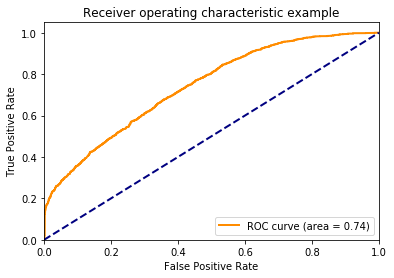
\includegraphics[width=2in,height=2in]{lstm4.png}}
            \caption{Receiver Operating Characteristic Curve Long Short Term Memory.}
            \end{figure}
        \end{column}
        \begin{column}{5cm}
            \begin{figure}[h]
            \centerline{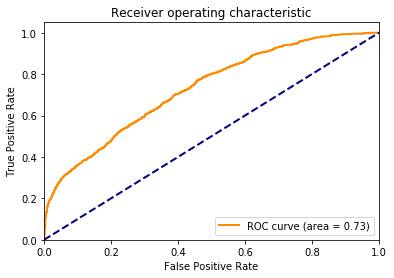
\includegraphics[width=2in,height=2in]{lstm_auto_encoder4.png}}
            \caption{Receiver Operating Characteristic Curve Long Short Term Memory Auto Encoders.}
            \end{figure}
        \end{column}
    \end{columns} 
    
\end{frame}

\begin{frame}{Preliminary Testing and Results Obtained\\ \footnotesize{Receiver Operating Curves}}
    \begin{columns}
        \begin{column}{.5\textwidth}
            \begin{figure}[h]
            \centerline{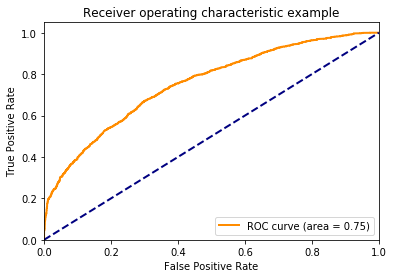
\includegraphics[width=2in,height=2in]{clstm4.png}}
            \caption{Receiver Operating Characteristic Curve Convolution Long Short Term Memory.}
            \end{figure}
        \end{column}
        \begin{column}{5cm}
            \begin{figure}[h]
            \centerline{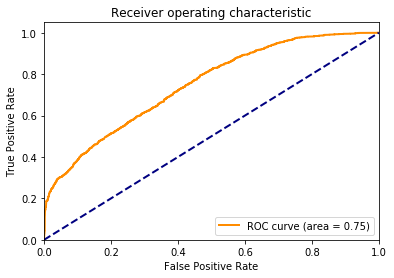
\includegraphics[width=2in,height=2in]{lstm-batalgorithm3.png}}
            \caption{Receiver Operating Characteristic Curve Long Short Term Memory with Bat Algorithm.}
            \end{figure}
        \end{column}
    \end{columns} 
    
\end{frame}

\begin{frame}{Preliminary Testing and Results Obtained\\ \footnotesize{Receiver Operating Curves}}
    \begin{figure}[h]
    \centerline{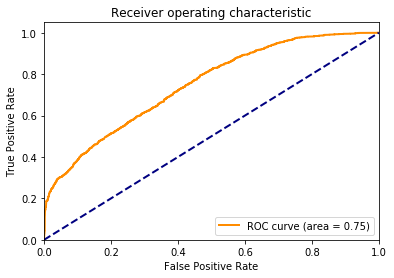
\includegraphics[width=2in,height=2in]{lstm-batalgorithm3.png}}
    \caption{Receiver Operating Characteristic Curve Convolution Long Short Term Memory with Grey Wolf Optimizer Algorithm.}
    \end{figure}
    
\end{frame}



\begin{frame}[allowframebreaks]{References}
%Sample reference file 
\bibliography{ref_ppt}
\nocite{*}
\end{frame}

\end{document}
